% Created by tikzDevice version 0.9 on 2015-12-18 02:49:03
% !TEX encoding = UTF-8 Unicode
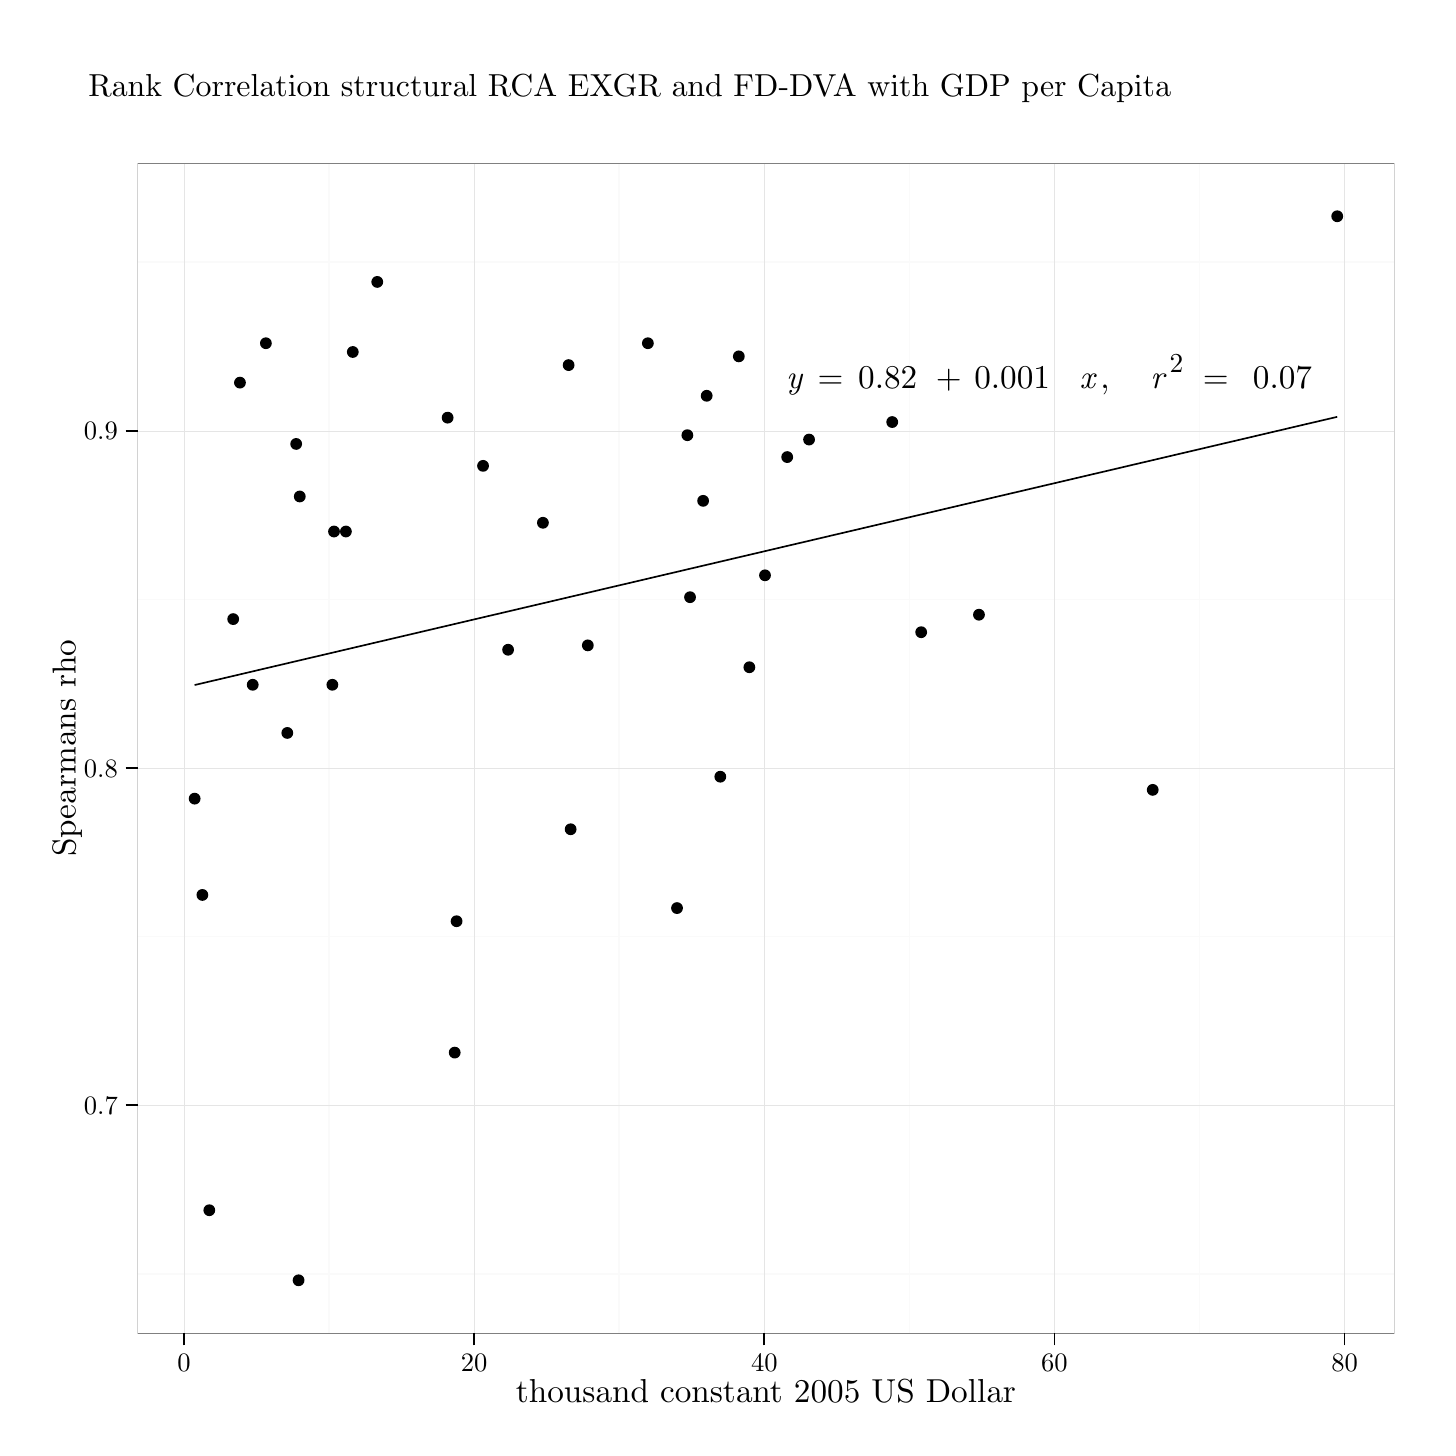
\begin{tikzpicture}[x=1pt,y=1pt]
\definecolor{fillColor}{RGB}{255,255,255}
\path[use as bounding box,fill=fillColor,fill opacity=0.00] (0,0) rectangle (505.89,505.89);
\begin{scope}
\path[clip] (  0.00,  0.00) rectangle (505.89,505.89);
\definecolor{drawColor}{RGB}{255,255,255}
\definecolor{fillColor}{RGB}{255,255,255}

\path[draw=drawColor,line width= 0.6pt,line join=round,line cap=round,fill=fillColor] (  0.00,  0.00) rectangle (505.89,505.89);
\end{scope}
\begin{scope}
\path[clip] ( 39.69, 34.03) rectangle (493.85,456.97);
\definecolor{fillColor}{RGB}{255,255,255}

\path[fill=fillColor] ( 39.69, 34.03) rectangle (493.85,456.97);
\definecolor{drawColor}{gray}{0.98}

\path[draw=drawColor,line width= 0.6pt,line join=round] ( 39.69, 55.63) --
	(493.85, 55.63);

\path[draw=drawColor,line width= 0.6pt,line join=round] ( 39.69,177.46) --
	(493.85,177.46);

\path[draw=drawColor,line width= 0.6pt,line join=round] ( 39.69,299.30) --
	(493.85,299.30);

\path[draw=drawColor,line width= 0.6pt,line join=round] ( 39.69,421.13) --
	(493.85,421.13);

\path[draw=drawColor,line width= 0.6pt,line join=round] (108.93, 34.03) --
	(108.93,456.97);

\path[draw=drawColor,line width= 0.6pt,line join=round] (213.76, 34.03) --
	(213.76,456.97);

\path[draw=drawColor,line width= 0.6pt,line join=round] (318.60, 34.03) --
	(318.60,456.97);

\path[draw=drawColor,line width= 0.6pt,line join=round] (423.43, 34.03) --
	(423.43,456.97);
\definecolor{drawColor}{gray}{0.90}

\path[draw=drawColor,line width= 0.2pt,line join=round] ( 39.69,116.55) --
	(493.85,116.55);

\path[draw=drawColor,line width= 0.2pt,line join=round] ( 39.69,238.38) --
	(493.85,238.38);

\path[draw=drawColor,line width= 0.2pt,line join=round] ( 39.69,360.21) --
	(493.85,360.21);

\path[draw=drawColor,line width= 0.2pt,line join=round] ( 56.51, 34.03) --
	( 56.51,456.97);

\path[draw=drawColor,line width= 0.2pt,line join=round] (161.34, 34.03) --
	(161.34,456.97);

\path[draw=drawColor,line width= 0.2pt,line join=round] (266.18, 34.03) --
	(266.18,456.97);

\path[draw=drawColor,line width= 0.2pt,line join=round] (371.02, 34.03) --
	(371.02,456.97);

\path[draw=drawColor,line width= 0.2pt,line join=round] (475.85, 34.03) --
	(475.85,456.97);
\definecolor{fillColor}{RGB}{0,0,0}

\path[fill=fillColor] ( 86.08,391.86) circle (  2.13);

\path[fill=fillColor] (234.64,187.75) circle (  2.13);

\path[fill=fillColor] (256.97,387.11) circle (  2.13);

\path[fill=fillColor] (250.28,235.22) circle (  2.13);

\path[fill=fillColor] ( 76.71,377.62) circle (  2.13);

\path[fill=fillColor] ( 81.32,268.44) circle (  2.13);

\path[fill=fillColor] (245.36,372.87) circle (  2.13);

\path[fill=fillColor] (343.75,293.76) circle (  2.13);

\path[fill=fillColor] ( 97.02,355.47) circle (  2.13);

\path[fill=fillColor] ( 65.63, 78.57) circle (  2.13);

\path[fill=fillColor] ( 74.26,292.18) circle (  2.13);

\path[fill=fillColor] (186.18,326.98) circle (  2.13);

\path[fill=fillColor] (126.32,414.01) circle (  2.13);

\path[fill=fillColor] (238.38,358.63) circle (  2.13);

\path[fill=fillColor] (312.40,363.38) circle (  2.13);

\path[fill=fillColor] (195.47,383.95) circle (  2.13);

\path[fill=fillColor] (110.70,323.82) circle (  2.13);

\path[fill=fillColor] (260.78,274.77) circle (  2.13);

\path[fill=fillColor] (239.34,300.09) circle (  2.13);

\path[fill=fillColor] (266.43,308.00) circle (  2.13);

\path[fill=fillColor] (173.60,281.10) circle (  2.13);

\path[fill=fillColor] (196.20,216.23) circle (  2.13);

\path[fill=fillColor] (110.10,268.44) circle (  2.13);

\path[fill=fillColor] (114.99,323.82) circle (  2.13);

\path[fill=fillColor] ( 63.13,192.50) circle (  2.13);

\path[fill=fillColor] ( 60.33,227.30) circle (  2.13);

\path[fill=fillColor] (322.87,287.43) circle (  2.13);

\path[fill=fillColor] (164.55,347.55) circle (  2.13);

\path[fill=fillColor] (224.11,391.86) circle (  2.13);

\path[fill=fillColor] (244.07,334.90) circle (  2.13);

\path[fill=fillColor] (154.31,135.53) circle (  2.13);

\path[fill=fillColor] (473.20,437.74) circle (  2.13);

\path[fill=fillColor] ( 97.89, 53.26) circle (  2.13);

\path[fill=fillColor] (274.45,350.72) circle (  2.13);

\path[fill=fillColor] (406.53,230.47) circle (  2.13);

\path[fill=fillColor] (202.41,282.68) circle (  2.13);

\path[fill=fillColor] ( 98.32,336.48) circle (  2.13);

\path[fill=fillColor] (154.98,183.00) circle (  2.13);

\path[fill=fillColor] (117.48,388.69) circle (  2.13);

\path[fill=fillColor] (151.75,364.96) circle (  2.13);

\path[fill=fillColor] (282.35,357.05) circle (  2.13);

\path[fill=fillColor] ( 93.82,251.04) circle (  2.13);
\definecolor{drawColor}{RGB}{0,0,0}

\path[draw=drawColor,line width= 0.6pt,line join=round] ( 60.33,268.35) --
	( 65.56,269.58) --
	( 70.78,270.80) --
	( 76.01,272.03) --
	( 81.24,273.26) --
	( 86.46,274.49) --
	( 91.69,275.71) --
	( 96.91,276.94) --
	(102.14,278.17) --
	(107.37,279.39) --
	(112.59,280.62) --
	(117.82,281.85) --
	(123.04,283.07) --
	(128.27,284.30) --
	(133.50,285.53) --
	(138.72,286.75) --
	(143.95,287.98) --
	(149.18,289.21) --
	(154.40,290.43) --
	(159.63,291.66) --
	(164.85,292.89) --
	(170.08,294.11) --
	(175.31,295.34) --
	(180.53,296.57) --
	(185.76,297.79) --
	(190.99,299.02) --
	(196.21,300.25) --
	(201.44,301.47) --
	(206.66,302.70) --
	(211.89,303.93) --
	(217.12,305.15) --
	(222.34,306.38) --
	(227.57,307.61) --
	(232.80,308.83) --
	(238.02,310.06) --
	(243.25,311.29) --
	(248.47,312.51) --
	(253.70,313.74) --
	(258.93,314.97) --
	(264.15,316.19) --
	(269.38,317.42) --
	(274.61,318.65) --
	(279.83,319.87) --
	(285.06,321.10) --
	(290.28,322.33) --
	(295.51,323.55) --
	(300.74,324.78) --
	(305.96,326.01) --
	(311.19,327.23) --
	(316.41,328.46) --
	(321.64,329.69) --
	(326.87,330.91) --
	(332.09,332.14) --
	(337.32,333.37) --
	(342.55,334.59) --
	(347.77,335.82) --
	(353.00,337.05) --
	(358.22,338.27) --
	(363.45,339.50) --
	(368.68,340.73) --
	(373.90,341.95) --
	(379.13,343.18) --
	(384.36,344.41) --
	(389.58,345.63) --
	(394.81,346.86) --
	(400.03,348.09) --
	(405.26,349.31) --
	(410.49,350.54) --
	(415.71,351.77) --
	(420.94,352.99) --
	(426.17,354.22) --
	(431.39,355.45) --
	(436.62,356.67) --
	(441.84,357.90) --
	(447.07,359.13) --
	(452.30,360.35) --
	(457.52,361.58) --
	(462.75,362.81) --
	(467.98,364.03) --
	(473.20,365.26);

\node[text=drawColor,anchor=base west,inner sep=0pt, outer sep=0pt, scale=  1.2] at (274.09,375.51) {\itshape y};

\node[text=drawColor,anchor=base west,inner sep=0pt, outer sep=0pt, scale=  1.2] at (285.49,375.51) {=};

\node[text=drawColor,anchor=base west,inner sep=0pt, outer sep=0pt, scale=  1.2] at (300.12,375.51) {0.82};

\node[text=drawColor,anchor=base west,inner sep=0pt, outer sep=0pt, scale=  1.2] at (328.19,375.51) {+};

\node[text=drawColor,anchor=base west,inner sep=0pt, outer sep=0pt, scale=  1.2] at (342.09,375.51) {0.001};

\node[text=drawColor,anchor=base west,inner sep=0pt, outer sep=0pt, scale=  1.2] at (377.25,375.51) {};

\node[text=drawColor,anchor=base west,inner sep=0pt, outer sep=0pt, scale=  1.2] at (380.13,375.51) {\itshape x};

\node[text=drawColor,anchor=base west,inner sep=0pt, outer sep=0pt, scale=  1.2] at (387.62,375.51) {,};

\node[text=drawColor,anchor=base west,inner sep=0pt, outer sep=0pt, scale=  1.2] at (391.56,375.51) { };

\node[text=drawColor,anchor=base west,inner sep=0pt, outer sep=0pt, scale=  1.2] at (398.64,375.51) { };

\node[text=drawColor,anchor=base west,inner sep=0pt, outer sep=0pt, scale=  1.2] at (405.72,375.51) {\itshape r};

\node[text=drawColor,anchor=base west,inner sep=0pt, outer sep=0pt, scale=  0.99] at (412.61, 381.3) {2};

\node[text=drawColor,anchor=base west,inner sep=0pt, outer sep=0pt, scale=  1.2] at (417.57,375.51) { };

\node[text=drawColor,anchor=base west,inner sep=0pt, outer sep=0pt, scale=  1.2] at (424.65,375.51) {=};

\node[text=drawColor,anchor=base west,inner sep=0pt, outer sep=0pt, scale=  1.2] at (435.67,375.51) { };

\node[text=drawColor,anchor=base west,inner sep=0pt, outer sep=0pt, scale=  1.2] at (442.76,375.51) {0.07};
\definecolor{drawColor}{gray}{0.50}

\path[draw=drawColor,line width= 0.6pt,line join=round,line cap=round] ( 39.69, 34.03) rectangle (493.85,456.97);
\end{scope}
\begin{scope}
\path[clip] (  0.00,  0.00) rectangle (505.89,505.89);
\definecolor{drawColor}{RGB}{0,0,0}

\node[text=drawColor,anchor=base east,inner sep=0pt, outer sep=0pt, scale=  0.96] at ( 32.57,113.24) {0.7};

\node[text=drawColor,anchor=base east,inner sep=0pt, outer sep=0pt, scale=  0.96] at ( 32.57,235.07) {0.8};

\node[text=drawColor,anchor=base east,inner sep=0pt, outer sep=0pt, scale=  0.96] at ( 32.57,356.91) {0.9};
\end{scope}
\begin{scope}
\path[clip] (  0.00,  0.00) rectangle (505.89,505.89);
\definecolor{drawColor}{RGB}{0,0,0}

\path[draw=drawColor,line width= 0.6pt,line join=round] ( 35.42,116.55) --
	( 39.69,116.55);

\path[draw=drawColor,line width= 0.6pt,line join=round] ( 35.42,238.38) --
	( 39.69,238.38);

\path[draw=drawColor,line width= 0.6pt,line join=round] ( 35.42,360.21) --
	( 39.69,360.21);
\end{scope}
\begin{scope}
\path[clip] (  0.00,  0.00) rectangle (505.89,505.89);
\definecolor{drawColor}{RGB}{0,0,0}

\path[draw=drawColor,line width= 0.6pt,line join=round] ( 56.51, 29.77) --
	( 56.51, 34.03);

\path[draw=drawColor,line width= 0.6pt,line join=round] (161.34, 29.77) --
	(161.34, 34.03);

\path[draw=drawColor,line width= 0.6pt,line join=round] (266.18, 29.77) --
	(266.18, 34.03);

\path[draw=drawColor,line width= 0.6pt,line join=round] (371.02, 29.77) --
	(371.02, 34.03);

\path[draw=drawColor,line width= 0.6pt,line join=round] (475.85, 29.77) --
	(475.85, 34.03);
\end{scope}
\begin{scope}
\path[clip] (  0.00,  0.00) rectangle (505.89,505.89);
\definecolor{drawColor}{RGB}{0,0,0}

\node[text=drawColor,anchor=base,inner sep=0pt, outer sep=0pt, scale=  0.96] at ( 56.51, 20.31) {0};

\node[text=drawColor,anchor=base,inner sep=0pt, outer sep=0pt, scale=  0.96] at (161.34, 20.31) {20};

\node[text=drawColor,anchor=base,inner sep=0pt, outer sep=0pt, scale=  0.96] at (266.18, 20.31) {40};

\node[text=drawColor,anchor=base,inner sep=0pt, outer sep=0pt, scale=  0.96] at (371.02, 20.31) {60};

\node[text=drawColor,anchor=base,inner sep=0pt, outer sep=0pt, scale=  0.96] at (475.85, 20.31) {80};
\end{scope}
\begin{scope}
\path[clip] (  0.00,  0.00) rectangle (505.89,505.89);
\definecolor{drawColor}{RGB}{0,0,0}

\node[text=drawColor,anchor=base,inner sep=0pt, outer sep=0pt, scale=  1.20] at (266.77,  9.03) {thousand constant 2005 US Dollar};
\end{scope}
\begin{scope}
\path[clip] (  0.00,  0.00) rectangle (505.89,505.89);
\definecolor{drawColor}{RGB}{0,0,0}

\node[text=drawColor,rotate= 90.00,anchor=base,inner sep=0pt, outer sep=0pt, scale=  1.20] at ( 17.30,245.50) {Spearmans rho};
\end{scope}
\begin{scope}
\path[clip] (  0.00,  0.00) rectangle (505.89,505.89);
\definecolor{drawColor}{RGB}{0,0,0}

\node[text=drawColor,anchor=base west,inner sep=0pt, outer sep=0pt, scale=  1.15] at ( 21.89,480.92) {Rank Correlation structural RCA EXGR and FD-DVA with GDP per Capita};
\end{scope}
\end{tikzpicture}
